\chapter{Background}
\label{chap:background}
\setheader{Background}

In this chapter most of the theory about measuring the directivity of a smartphone microphone is addressed.
The related research will be discussed first, after which the operations of a beamforming algorithm is briefly explained, followed by a comparison between different sampling schemes for spherical sampling and methods to measure the impulse response.
Of these impulse response determination methods, two techniques will be explained in more detail, since they will be used in the measurements (further explanation of this choice is given in Chapter \ref{chap:measurements}).
In the next chapter, the final choices concerning the directivity measurements  will be made on base of this presented theory.   

\section{Related Research}
This research is a continuation of the work of Gaubitch et al. \cite{Gaubitch2014}, who concluded the directivity of a smartphone microphone could be used to improve beamforming algorithms.
While some smartphone directivity measurements were already conducted for this paper, these were only performed in a two-dimensional plane around the smartphone, instead of a full three-dimensional sphere \cite{Gaubitch2014}.
The smartphone available for the measurements is \nexus~ \cite{nexus5}.
No information about the microphone used in this mobile phone is made available by Google \cite{nexus5} or LG \cite{nexus5:lg}, the two parties that produced it.
Information about microphone control and automatic gain control from the smartphone is also not given \cite{BAP:RoySjoerd}.

Determining the directivity is, in short, determining the impulse response of the microphone with respect to signals from different directions.
This comes down to two parts: impulse response determination and sampling in space.
To take the measured directivities into account in the beamforming algorithm, the measured results must be converted to a more suitable form for the algorithm.
The directivities are measured for a certain number of data points. The beamforming algorithm also needs the directivities for an intermediate value, thus interpolation is necessary. 
These interpolation calculations will take time and computing power, a possible source of trouble in the beamforming algorithm \cite{BAP:ErikNiels}. 
The algorithm will use the information from the measurements multiple times per second \cite{BAP:ErikNiels}, so performing this interpolation during the actual beamforming is undesirable. Instead, all the interpolation is done as a preprocessing step as the algorithm only works with non-moving and known places in space \cite{BAP:ErikNiels}. As a result, when directivity data for a given orientation is requested, only a look-up is performed

In the next section, the operations of a beamforming algorithm is discussed, as well as how to account for the directivity of (for instance) a smartphone microphone in these algorithms.

\subsection{Beamforming}
\label{ssec:background-beamforming}
This thesis is about the directivity of a smartphone microphone, which is to be used in a beamforming algorithm.
It is therefore important to know more about beamforming in general, to specify the type of beamforming used in this research and to recognize the role of the microphone directivity in such an algorithm.  


Beamforming is a widely used technique in the field of signal processing with the purpose to transmit or receive signals directionally.
Several algorithms for achieving this goal are described in the literature \cite{mucci1984comparison}.
Beamforming makes use of an array of sensors to achieve spatial filtering \cite{VanVeen19884}.
A beamformer processes the spatial samples of propagating wave fields, collected by the sensor array.
Signals with overlapping frequency content but different spatial origin are separated.
Desired signals from a certain direction can then be estimated despite the presence of noise and interfering signals. 
In this way, the beamformer can select the desired signal and eliminate the undesired one. 

Because of the variety of beamforming applications, several distinctions have to be made to determine the type of beamforming in this project.
The beamforming discussed here is about voice signal reception with smartphone microphones.
Beamforming can be used with different types of sensor arrays. Sensor arrays may vary in geometry, number and size \cite{VanVeen19884}.
The array geometry could vary from linear, circular, spherical to arbitrary geometries.
This research focuses on so-called ad-hoc microphone arrays, which are microphone sensor arrays with arbitrary geometries \cite{BAP:ErikNiels}. 

Beamforming can be classified as either near-field or far-field, with different algorithms required for each. The situation depends on the dimensions of the array \cite{ryan1997near}.
If the wave field originates from a distance far greater than the dimensions of the array, the situation can be considered far-field.
There will be no difference in Direction of Arrival (DOA) for every sensor in the array, because the wave field can then be assumed to have a flat wave front.
However, in the case of near-field beamforming the distance between the source and the array is comparable to the dimensions of the array.
This will lead to a noticeable difference in DOA and amplitude of the signal at every sensor.  
During a conference call, the distance between the participant (source) and the smartphone microphone will be small. Therefore, this is considered a near-field scenario \cite{BAP:ErikNiels}. 

The last distinction to be made concerns the choice between broadband and narrowband beamforming techniques \cite{brandstein2001}. This choice depends on the signals incident on the array. The size of an array in terms of operating wavelength is important in measuring array performance. Consider a linear array with a fixed number of elements and fixed inter-element distance. For high frequency signals (with small wavelength) incident on the array, this fixed array will appear large and the main beam will be narrow. In case of low frequency signals (with large wavelength), this same array will appear small and the main beam appears wide. 
For application of the processed signals in speech communication the beamforming algorithm has to operate well in a frequency band from 300 Hz to 3500 Hz \cite{doclo2003design}.
A speech signal is a very wideband signal, which covers some four octaves. If a speech signal is used in a narrowband array, this will give a disturbing speech output. This is the result of a varying beam width caused by the wide frequency range. The interfering signal will not be uniformly attenuated but instead low-pass filtered over its entire band \cite{brandstein2001}. 
In speech applications the narrowband assumption is therefore never valid and a beamformer designed specifically for broadband applications need to be used. 

Beamforming with smartphone microphone arrays is a form of acoustic beamforming. It can be applied in a room with multiple speakers, which is the case during a conference call.
The desired signal originates from a speaker's mouth and is hindered by the signals caused by other speakers and room reverberation \cite{brandstein2001}.
In this case, spatial filtering can be applied because the interfering sources usually originate from points in space apart from the unwanted signal origins.
When the locations of the speakers and smartphones are known, the beamformer algorithm can be used to select the voices and sounds you want to hear and reject noise.

Each $i^\text{th}$ microphone in the array observes a signal $Y_{i}$($\omega$) of the form of equation \eqref{eq:beamformer}, with $S(\omega)$ is the desired voice signal. 
The presence of noise sources is indicated by $V_{i}$($\omega$).
The signal travels through the room and through the microphone, each affecting the desired signal. 
The acoustic transfer function of the room is given by $H_{i}(\omega)$ 
\cite{Gaubitch2014},
\begin{equation}
\label{eq:beamformer}
Y_{i}(\omega) = S(\omega) H_{i}(\omega) G_{i} (\omega,\theta,\phi) + V_{i}(\omega).
\end{equation}
The frequency response of the smartphone microphone can be defined by $G_i(\omega,\theta,\phi)$.
As can be seen, this frequency response depends on both the frequency and orientation of the smartphone microphone relative to the source (the orientation is the direction from which the signal arrives with respect to the speechside of the smartphone, given in $\phi$ and $\theta$).

This frequency \textit{and} orientation dependency of the microphone is called the microphone directivity. 
The directivity is related to how a microphone receives sounds from a source dependent on their relative orientation. 
An approaching signal will thus be recorded with different intensities, according to the side it comes from.
These differences need to be considered in the calculation of the weights by the beamforming algorithm \cite{Gaubitch2014,thomas2012optimal} . 
This thesis is about the microphone directivity, more details about the beamforming algorithms are given in \cite{BAP:ErikNiels}. 

\subsection{Sampling schemes}
\label{sec:rel_res:sampl_sch}
For determining the directivity of a microphone, the impulse response of the microphone will need to be determined for different points in space.
A logical sampling scheme (the placement of sampling points in space) is a sphere, with the smartphone in its center, for it has equal distances all sampling points to the smartphone.
The advantage of this is that there is no correction needed with respect to the attenuation because all distances are the same.

Sampling and interpolation methods on a sphere are rooted in non trivial mathematics \cite{Marzo2014}. Zhang et al.\ \cite{Zhang2012575} show that there exists a minimum number of measurement points $M$ on a sphere 
\begin{equation}
\label{eqn:minimum}
M\equiv\left\lceil\left(\dfrac{e\pi sf}{c}+1\right)^2\right\rceil.
\end{equation}
With $e=\exp(1)$, $s$ the radius of the sphere, $f$ the highest frequency of the signal to be measured and $c$ speed of sound.

Zhang et al.\ \cite{Zhang2012575} also describe and compare four different sampling schemes for a sphere: three existing sampling schemes and one developed by Zhang et al.\ \cite{Zhang2012575}, IGLOO, an example of the distribution of sampling points on a sphere using the IGLOO method can be found in Figure \ref{fig:IGLOO}, for which they took in consideration that it is desirable to keep the rotations to a minimum number of steps \cite{Zhang2012575}. Their results are given in Table \ref{tab:IGLOO}.

\begin{itemize}
\item[]	\textbf{Equiangular grid} is a grid equally divided in latitudes and longitudes. The biggest drawback is the overly densely sampled pole-region, which is reflected in the high number of samples needed compared with the ideal number.
\item[]	\textbf{Gauss-Legendre sampling} takes the points as roots of a Legendre polynomial and corresponding weights are determined by the Gauss-Legendre method. The downside of this method is that there is no regularity in the sampling region and that the sampling grids for different resolutions are completely dissimilar. As such, a lower-resolution sampling grid cannot simply be taken as a subset of a higher-resolution grid.
\item[]	\textbf{HEALPix} requires a lot of sample points with respect to the other three sampling methods and the stated minimum (equation \eqref{eqn:minimum}). Also, the azimuthal positions change with the elevation.
\item[]	\textbf{IGLOO} divides the sphere into a number of base regions subject to a minimum distortion criterion \cite{Zhang2012575}. The data posseses an exact discrete azimuthal symmetry which allows fast and precise spherical harmonic transform computation. The sample locations are more suitable for automatic measurement.
\end{itemize}

\begin{figure}[t!]
    \centering
    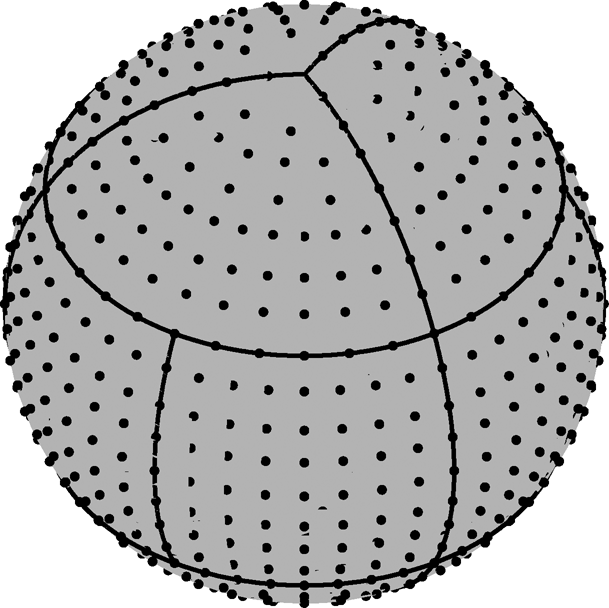
\includegraphics[width=5cm]{afbeeldingen/Directivity_IGLOO.png}
    \caption[IGLOO sampling scheme from \cite{Zhang2012575}]{An example of a IGLOO sampling scheme, Fig. 1 from \cite{Zhang2012575}. \textit{Picture of the 3:6:3 equal area division, which divides the sphere into 12 base regions, three at either cap and six $60^\circ\times60^\circ$ equatorial regions. Here, each base region is sampled with 64 points.}}
    \label{fig:IGLOO}
\end{figure}

\begin{table}[t]
\centering
\begin{tabular}{ccccc}
\hline
\hline
&Equiangular&Gauss-Legendre&HEALPix&IGLOO\\
\hline
Number of samples (for 20 kHz bandwidth)&8836&4371&12288&3072\\
Equal area division&No&No&Yes&Almost\\
Hierarchical&Yes&No&Yes&Yes\\
Iso-longitude&Yes&Yes&No&No\\
\hline
\hline
\end{tabular}
\caption{Comparison between four different methods for sampling on a sphere, Table I from \cite{Zhang2012575}. The ideal number of samples is 2209.}
\label{tab:IGLOO}
\end{table}

Very recently new research on grid sampling on spheres has been done\footnote{These papers will be published in the proceedings of the International Conference on Acoustics, Speech and Signal Processing 2015 (ICASSP'2015), which took place after the start of the Bachelor Graduation Project.}
\cite{bates2015optimal,khalidspherical}, which might provide an improvement in following work.

\subsection{Interpolation}
The resulting impulse responses can be labelled with two dimensions: an elevation $\phi$ and an azimuth $\theta$.
The complex gain of a signal however is also dependent on frequency.
This complex gain can be determined by using the Fourier transform of the impulse response.
Interpolation is needed to find the impulse response on a full sphere.
However \cite{goslinski2015performance,BAP:RoySjoerd} the azimuth and elevation determination of a modern smartphone is not so precise.
It often differs more than $10^\circ$.
Therefore interpolation in the spatial domain is not a great concern. The $\phi$ and $\theta$ error due to imprecise orientation measurement outweighs the error caused by nearest-neighbour interpolation.
It would be a waste of time to compute the complex gain for a given spatial coordinates, which probably differ about $10^\circ$ from the real place.

Interpolation in the frequency domain can be done using the reconstruction formula \cite[p.~420]{book:dsp} (example with the spectrum $X(\omega)$ of the sequence $x[n]$ in \eqref{eqn:reconstruction_formula}), which provides a properly weighted linear combination of the original spectral samples.
This can be performed more easily using a technique called zero-padding \cite[p.~420-425]{book:dsp}, where zeros are added to the end of the time-domain signal before  transformation to the Fourier domain.
Zero padding does not introduce any new information about the frequency content of the signal, it merely serves to interpolate the spectrum to the desired size.
The zero padding will be done in the beamforming algorithm, explained in Chapter \ref{chap:implementation},

\begin{equation}
\label{eqn:reconstruction_formula}
\begin{split}
X[\omega]&=\mathlarger\sum\limits_{k=0}^{N-1}X\left[\dfrac{2\pi}{N}k\right]P\left[\omega-\dfrac{2\pi}{N}k\right]\\
P\left[\dfrac{2\pi}{N}k\right]&=
\left\{
\begin{array}{ll}
1,&k=0\\
0,&k=1,2,\ldots,N-1.
\end{array}
\right.
\end{split}
\end{equation}


%----------------------------------------------------------------------------------
\subsection{Impulse response}
The response of a system to a single impulse (Delta pulse, discussed later) is called the impulse response of a system.
The impulse response of a smartphone microphone is assumed to be \textit{linear} and time-invariant, so it can be described by a linear and time-invariant system (LTI system) \cite[p.~17]{girod2001signals} \cite{Thomas2006, Stan2002249}.
This assumption is made because the source (loudspeaker) and receiver (microphone) are in a fixed place during each measurement and the smartphone is not exposed to significant temperature changes.
 
A property of an LTI system is that its behaviour can be characterized by its impulse response \cite[p.~105]{book:dsp}.
This means that for a given input signal, the output signal can be calculated using the impulse response of the system.
This also implies that the impulse response can be found by a convolution of a known input signal and a measured output signal.  
The frequency response of a system is the Fourier transform of the impulse response and the other way around.
The input signal and corresponding deconvolution technique should give the deconvolved impulse response a maximized signal-to-noise ratio \cite{Stan2002249}. 
It is desirable to know the behaviour, and thus to find the impulse response, of the smartphone microphone for a wide range of frequencies.
It is therefore necessary to use an input test signal that contains many frequencies equally. 

The theoretically most simple signal to use for impulse response measurements in continuous time is the Dirac delta pulse $\delta(t-\tau)$ \cite[p.~158-159]{girod2001signals} \eqref{eq:delta}, in digital signal processing the unit sample sequence $\delta[n]$ is most often used \cite[p.~42]{book:dsp} \eqref{eq:delta_dig}.
This is a hypothetical distribution representing an infinitely high impulse of infinitesimal duration, giving it a flat power spectrum - it contains all frequencies equally.

Convolution of the Dirac delta with a function yields the function that was convolved with it, and as such an impulse response is directly usable for modelling the response of a system \cite[p.~169-171]{girod2001signals}.
Unfortunately, the Dirac delta is only a hypothetical distribution.
Real approximations to it suffer from a very large dynamic range (the ratio between the smallest and largest amplitude of the signal) - the signal power is very localised in time, which makes it difficult to put enough power into the pulse for adequate signal-to-noise ratio (S/N) \cite{hee2003}

\begin{eqnarray}
\label{eq:delta}\delta(t-\tau)&=&\left\{\begin{array}{cl}
\infty&\text{for }t=\tau\\
0&\text{elsewhere,}
\end{array}\right.\qquad\text{with: }\int\limits_{-\infty}^\infty\delta(t)\text{ d}t=1,\\
\label{eq:delta_dig}\delta[n]&=&\left\{\begin{array}{cl}
1&\text{for }n=0\\
0&\text{elsewhere.}
\end{array}\right.
\end{eqnarray}

The following three discussed impulse response methods aim to keep the flat power spectrum of the Dirac delta, while trying to improve on its dynamic range behaviour. 
They are commonly used methods for measuring impulse responses.
The three impulse response measurement methods taken into account in this work are maximum length sequences (MLS) \cite{hee2003}, time stretched pulses (TSP) \cite{Aoshima19811484} and the sine sweep technique \cite{Stan2002249}. 

\section{Impulse response measurement methods}
These three techniques have different advantages and disadvantages, as compared by Stan et al. \cite{Stan2002249} and Thomas \cite{Thomas2006}.
The MLS technique is strongly immune to all kinds of noise and it has a relatively low optimal sound level \cite{Stan2002249}.
The TSP technique on the other hand is much less sensitive to distortion by non-linearities than the MLS technique \cite{Stan2002249}, but is much less suited for noisy environments.

The Sine Sweep technique is concluded to be the best method for impulse response measurements in quiet rooms by Stan et al. \cite{Stan2002249}.
It is insensitive to harmonic distortion and has an excellent signal-to-noise ratio.
Its calibration is a lot less tedious to obtain good results, but is not recommended for measurements in noisy environments.
However, Thomas \cite{Thomas2006} notes that the Sine Sweep technique concentrates excitation energy to a very narrow spectrum. Because speech does not tend to contain single tones, the sine sweep technique is less useful for applications in speech.
In addition, the sine sweep technique does not yield phase information \cite{Thomas2006}.
The phase information can be used by the beamforming algorithm, so the sine sweep technique does not seem appropriate for the intended purpose, therefore this technique will not be discussed any further. 

\subsection{Time Stretched Pulse (TSP)}
The time-stretched pulse (TSP) technique is an impulse response measurement method which was introduced by Aoshima \cite{Aoshima19811484}.
It is based on specifying a wideband, spectrally flat signal, then taking the inverse Fourier transform to yield a suitable time-domain signal.
If the phase of the signal is taken to be zero, an impulse-like signal results which, as discussed above, is unsuitable for practical applications.
The time-stretched pulse can be considered to be the output of a phase-shifting filter applied to an impulse signal, with a transfer function given by
\begin{equation}
H[\omega] = \exp[j(12\omega^{2}/10000)].
\label{eq:TSPfilter}
\end{equation}
The numbers in this equation are chosen such that this filter has a magnitude of 1, so it will conserve the wideband frequency content of the signal and only shift its phase.
This added phase shift results in a stretched signal in time.
The impulse response can be recovered by using an inverse filter with transfer function \eqref{eq:TSPinversefilter} on the Fourier transform of the received signal
\begin{equation}
H^{-1}[\omega] = \exp[-j(12\omega^{2}/10000)].
\label{eq:TSPinversefilter}
\end{equation}
The technique of Aoshima is suitable for sound signals with small time duration.
For long impulse responses, Aoshima's technique exhibits a discontinuity at frequencies over $f_{s}/2$ (with $f_s$ the sampling frequency) and below zero, which is caused by aliasing.
As the transfer functions of acoustic arrangements often display long impulse responses, Suzuki et al. \cite{Suzuki19951119} designed the Optimized Aoshima Time Stretched Pulse technique (OATSP).
They first generalized Aoshima's TSP to the function
\begin{equation}
\label{eqn:OATSPorigineel}
H[k]=\left\{
\begin{array}{ll}
\exp(jpk^2)& 0 \leq k < N/2\\
1&k=N/2\\
H^{*} [N-k] & N/2 < k < N.
\end{array}
\right.
\end{equation}    
Where $N=2^{i}$, with $i\in\mathbb{N}$, and the variable $p$ determines the stretch of the signal. 
Discontinuities in phase can arise because $H(N/2)$ is always set to the real value 1.
To remove this discontinuity, they introduced an integer $m$ that determines the stretch of the pulse, given by equation \eqref{eq:OATSPm}, which is then substituted in equation \eqref{eqn:OATSPorigineel}.
As can be seen from equation \eqref{eq:OATSP}, this integer $m$ prevents the occurrence of $H(N/2) = 1$ and thus removes the discontinuities.
The OATSP gives an almost ideal characteristic to measure impulse responses shorter and even longer than its specific length N.
The code to generate and analyse the TSP sequences, by Thomas \cite{Thomas2006}, uses this OATSP method:

\begin{eqnarray}
\label{eq:OATSPm} p[N/2]^{2} &=& m \pi\\
\label{eq:OATSP} H[k]&=&\left\{
\begin{array}{ll}
\exp(j4m \pi k^{2}/N^{2})& 0 \leq k \leq N/2\\
H^{*} [N-k] & N/2 < k < N.
\end{array}
\right.
\end{eqnarray}

\clearpage
\subsection{Maximum Length Sequence (MLS)}
A maximum length sequence is a pseudorandom two-level signal consisting of values +1 and -1, commonly generated by a linear feedback shift-register (LFSR).
The binary value 0 and 1 are mapped to -1 and +1 respectively \cite{hee2003}.
The signal is periodic with a period $P=2^N-1$ with N the number of bits: $N\in\mathbb{N}$.
The frequency behaviour of an MLS signal is flat, except for a small DC offset \cite{Thomas2006}.

Figure \ref{fig:register} illustrates an implementation of a LSFR as a block diagram. 
The LFSR repeatedly applies an exclusive or (XOR) operation on two coefficients.
The chosen coefficients can be calculated from a mathematical derived recursive formula.
After each XOR operation, the LFSR shifts a bit and performs the operation again. 
The LFSR initializes with N ones or N random numbers. 
This method has a good S/N ratio, which makes it suited for measurements in noisy environments \cite{hee2003}. 

Assume $s[n]$ to be the MLS input signal of the system and $x[n]$ ato bes the output signal of the system, with $h[n]$ the impulse response of the system.
When circular convolution \eqref{eq:circ_conv} \cite[p.~439]{book:dsp} is applied on the output of this system, the impulse response of the system can be obtained.
This is because the cross-correlation of $s[n]$ and $x[n]$ (defined as \eqref{eq:crosscor} \cite[p.~228-229]{girod2001signals}) has the same result as the circular convolution.
If the input and output signals are the same ($x[n]=s[n]$), the cross correlation of these signals approaches the Delta-function with a scaling factor $c$ \eqref{eq:todelta}.
Because $(s*h)[n]=x[n]$ and from this follows \eqref{eq:tada_ir}: in this way the circular convolution can be used to find the impulse response, differing from the real one by a scaling factor;

\begin{eqnarray}
\label{eq:circ_conv}
h[m]&=&\sum\limits_{n=0}^{N-1}s[n]x[m-n]\qquad m=0,1,\ldots,N-1\\
\label{eq:crosscor}
\text{crosscor}(s,x)[n]&=&s[-n]*x[n]\\
&=&\sum\limits_{m=-\infty}^\infty s[m]x[m-n] \nonumber \\
\label{eq:todelta}
\text{crosscor}(s,s)[n]&\approx&c\cdot\delta[n]\\
\label{eq:tada_ir}
\text{crosscor}(s,(s*h))[n]&=&s[-n]*(s*h)[n]=s[-n]*s*h\\
&\approx& c\cdot\delta*h=c\cdot h \nonumber.
\end{eqnarray}

\begin{figure}[h]
    \centering
    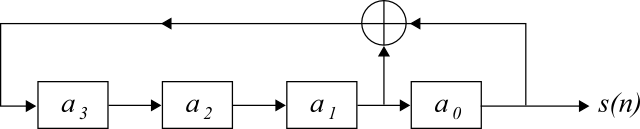
\includegraphics[width=10cm]{afbeeldingen/Directivity_MLS.png}
    \caption[MLS feedback shift-register]{A block diagram of a fourth order MLS, with $a_i$ the coefficients. The addition is modulo 2 (equivalent to the exclusive-or operation).}
    \label{fig:register}
\end{figure}

\section*{Background - Conclusion}
In this chapter first some related research was addressed.
This research is a continuation of Gaubitch et al. \cite{Gaubitch2014}; they concluded the directivity of a smartphone microphone could improve beamforming algorithms.
The inner working of these beamforming algorithms was explained, and the choice for an ad-hoc near-field broadband beamformer was elucidated.
After that, different sampling schemes on a sphere were presented with their advantages and disadvantages.
Finally three different impulse response determination methods were compared, and it was concluded that the Maximum Length Sequence and Time-Stretched Pulse techniques are more appropriate for the intended purpose than the Sine Sweep technique and therefore those two were explained in more detail.
